\section{Register description}
\regover{
{\hyperref[ausolo-audpdm-top]{audpdm\_top}}&Clock control register
\\
\hline
{\hyperref[ausolo-audpdm-itf]{audpdm\_itf}}&Interface control register 1
\\
\hline
{\hyperref[ausolo-pdm-adc-0]{pdm\_adc\_0}}&Filter control register 1
\\
\hline
{\hyperref[ausolo-pdm-adc-1]{pdm\_adc\_1}}&Filter control register 2
\\
\hline
{\hyperref[ausolo-pdm-dac-0]{pdm\_dac\_0}}&Interface control register 2
\\
\hline
{\hyperref[ausolo-pdm-pdm-0]{pdm\_pdm\_0}}&pdm control register
\\
\hline
{\hyperref[ausolo-pdm-adc-s0]{pdm\_adc\_s0}}&volume control register
\\
\hline
{\hyperref[ausolo-audadc-ana-cfg1]{audadc\_ana\_cfg1}}&ADC analog control register 1
\\
\hline
{\hyperref[ausolo-audadc-ana-cfg2]{audadc\_ana\_cfg2}}&ADC analog control register 2
\\
\hline
{\hyperref[ausolo-audadc-cmd]{audadc\_cmd}}&ADC control register
\\
\hline
{\hyperref[ausolo-audadc-data]{audadc\_data}}&measuring mode control register
\\
\hline
{\hyperref[ausolo-audadc-rx-fifo-ctrl]{audadc\_rx\_fifo\_ctrl}}&fifo control register
\\
\hline
{\hyperref[ausolo-audadc-rx-fifo-status]{audadc\_rx\_fifo\_status}}&fifo status register
\\
\hline
{\hyperref[ausolo-audadc-rx-fifo-data]{audadc\_rx\_fifo\_data}}&fifo data register
\\
\hline
}

\subsection{audpdm\_top}
\label{ausolo-audpdm-top}
Address:0x2000ac00
 \begin{figure}[H]
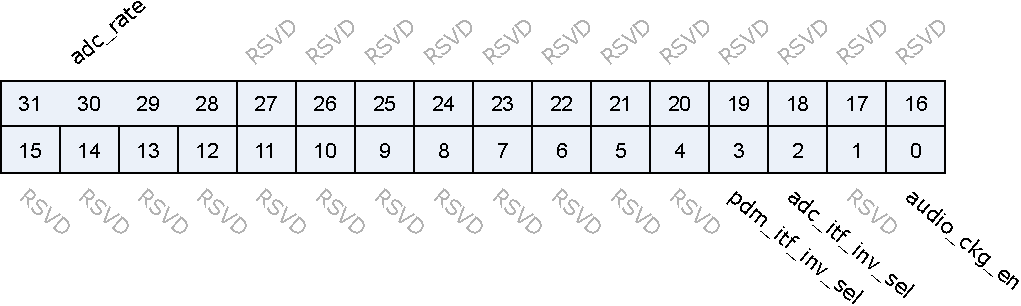
\includegraphics{ausolo_audpdm_top.pdf}
\end{figure}

\regdes{31:4&RSVD& & & \\\hline
3&pdm\_itf\_inv\_sel&r/w&1'd0&invert clk\_pdm\\\hline
2&adc\_itf\_inv\_sel&r/w&1'd0&invert clk\_adc\\\hline
1&RSVD& & & \\\hline
0&audio\_ckg\_en&r/w&1'd0&enable audio clock generator\\\hline

}
\subsection{audpdm\_itf}
\label{ausolo-audpdm-itf}
Address:0x2000ac04
 \begin{figure}[H]
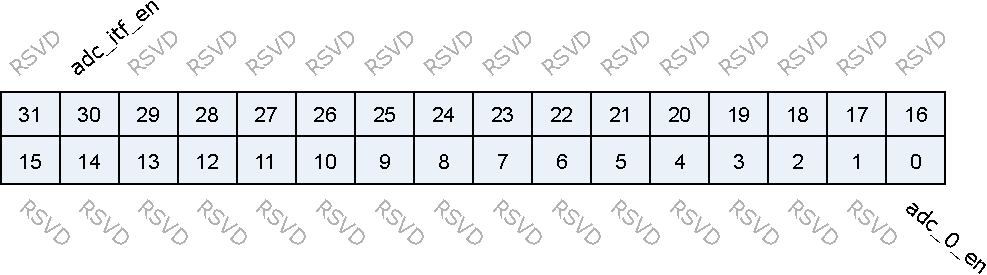
\includegraphics{ausolo_audpdm_itf.pdf}
\end{figure}

\regdes{31&RSVD& & & \\\hline
30&adc\_itf\_en&r/w&1'd0&enable adc to audio dma interface\\\hline
29:1&RSVD& & & \\\hline
0&adc\_0\_en&r/w&1'd0&enable adc\\\hline

}
\subsection{pdm\_adc\_0}
\label{ausolo-pdm-adc-0}
Address:0x2000ac08
 \begin{figure}[H]
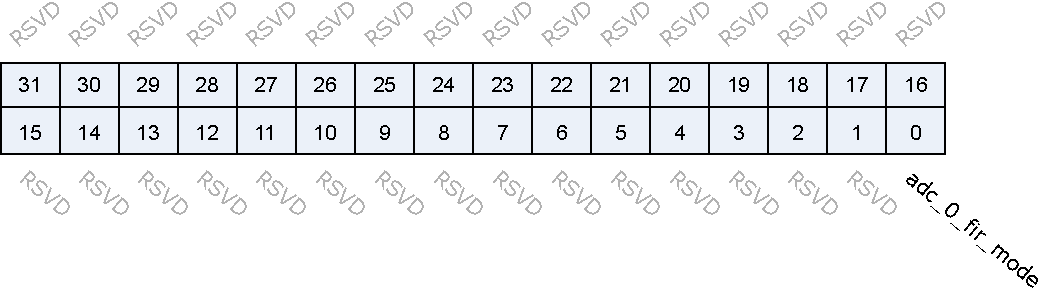
\includegraphics{ausolo_pdm_adc_0.pdf}
\end{figure}

\regdes{31:1&RSVD& & & \\\hline
0&adc\_0\_fir\_mode&r/w&1'd0&adc fir mode\\\hline

}
\subsection{pdm\_adc\_1}
\label{ausolo-pdm-adc-1}
Address:0x2000ac0c
 \begin{figure}[H]
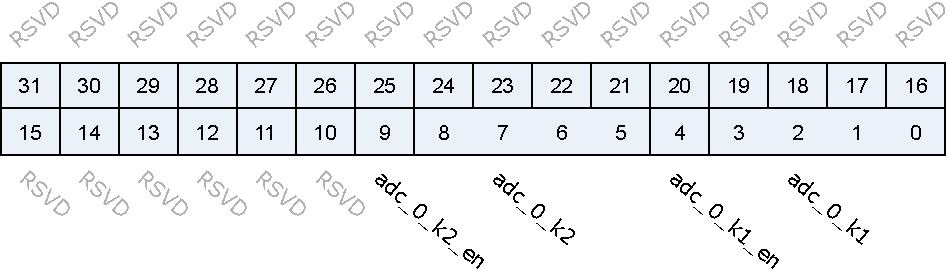
\includegraphics{ausolo_pdm_adc_1.pdf}
\end{figure}

\regdes{31:10&RSVD& & & \\\hline
9&adc\_0\_k2\_en&r/w&1'd0&adc ch0 hpf parameter k2 enable\\\hline
8:5&adc\_0\_k2&r/w&4'd13&adc ch0 hpf parameter k2\\\hline
4&adc\_0\_k1\_en&r/w&1'd1&adc ch0 hpf parameter k1 enable\\\hline
3:0&adc\_0\_k1&r/w&4'd8&adc ch0 hpf parameter k1\\\hline

}
\subsection{pdm\_dac\_0}
\label{ausolo-pdm-dac-0}
Address:0x2000ac10
 \begin{figure}[H]
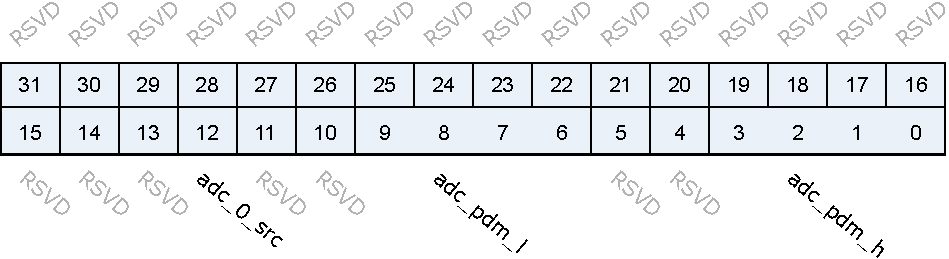
\includegraphics{ausolo_pdm_dac_0.pdf}
\end{figure}

\regdes{31:13&RSVD& & & \\\hline
12&adc\_0\_src&r/w&1'd0&0:adc mode, 1:pdm mode\\\hline
11:10&RSVD& & & \\\hline
9:6&adc\_pdm\_l&r/w&4'b1010&pdm low value\\\hline
5:4&RSVD& & & \\\hline
3:0&adc\_pdm\_h&r/w&4'b0110&pdm high value\\\hline

}
\subsection{pdm\_pdm\_0}
\label{ausolo-pdm-pdm-0}
Address:0x2000ac1c
 \begin{figure}[H]
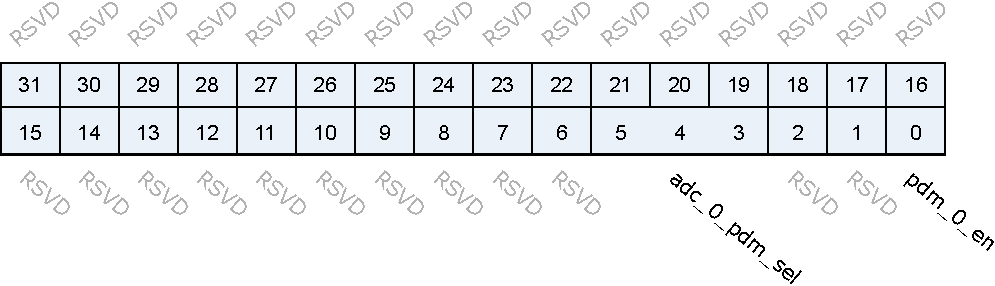
\includegraphics{ausolo_pdm_pdm_0.pdf}
\end{figure}

\regdes{31:6&RSVD& & & \\\hline
5:3&adc\_0\_pdm\_sel&r/w&3'd0&adc ch0 source select: 0:pdm\_l, 1:pdm\_r\\\hline
2:1&RSVD& & & \\\hline
0&pdm\_0\_en&r/w&1'd0&enable pdm\\\hline

}
\subsection{pdm\_adc\_s0}
\label{ausolo-pdm-adc-s0}
Address:0x2000ac38
 \begin{figure}[H]
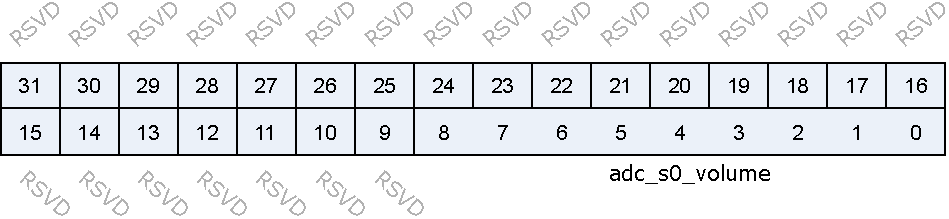
\includegraphics{ausolo_pdm_adc_s0.pdf}
\end{figure}

\regdes{31:9&RSVD& & & \\\hline
8:0&adc\_s0\_volume&r/w&9'd0&volume s9.1, -95.5dB ~ +18dB in 0.5dB step\\\hline

}
\subsection{audadc\_ana\_cfg1}
\label{ausolo-audadc-ana-cfg1}
Address:0x2000ac60
 \begin{figure}[H]
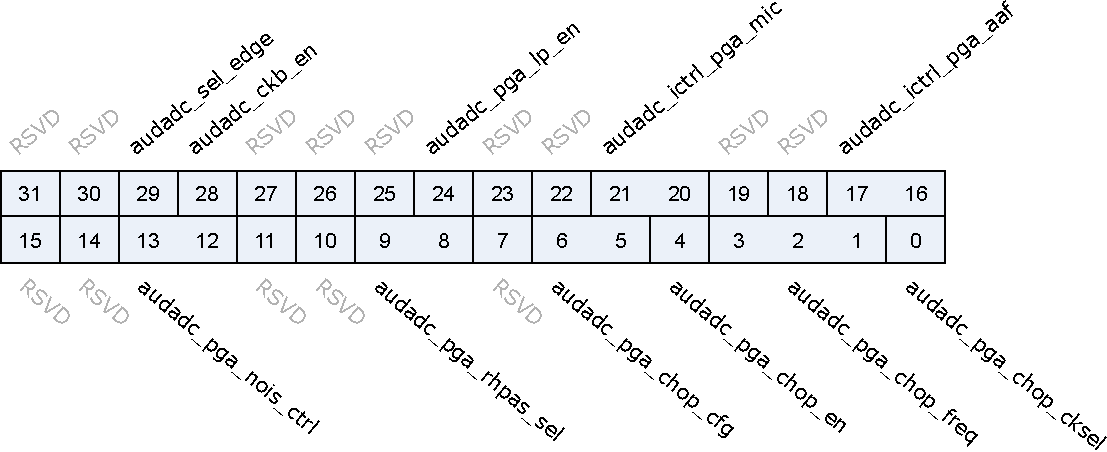
\includegraphics{ausolo_audadc_ana_cfg1.pdf}
\end{figure}

\regdes{31:30&RSVD& & & \\\hline
29&audadc\_sel\_edge&r/w&1'h0&ADC output data clock edge \par 0 = falling edge sent, rising edge recieve     \par 1 = rising edge sent, falling edge recieve 
\\\hline
28&audadc\_ckb\_en&r/w&1'h0&AUDADC clock phase control \par 0 = 0°        1 = 180° 
\\\hline
27:25&RSVD& & & \\\hline
24&audadc\_pga\_lp\_en&r/w&1'h0&PGA lowpower funciton \par reversed, not realized in circuit
\\\hline
23:22&RSVD& & & \\\hline
21:20&audadc\_ictrl\_pga\_mic&r/w&2'h1&PGA\_OPMIC bias current control \par 00 = 4uA          01 = 5uA \par 10 = 6uA          11 = 7uA
\\\hline
19:18&RSVD& & & \\\hline
17:16&audadc\_ictrl\_pga\_aaf&r/w&2'h1&PGA\_OPAAF bias current control \par 00 = 4uA          01 = 5uA \par 10 = 6uA          11 = 7uA
\\\hline
15:14&RSVD& & & \\\hline
13:12&audadc\_pga\_nois\_ctrl&r/w&2'h0&PGA noise control when configured to single-ended \par not used
\\\hline
11:10&RSVD& & & \\\hline
9:8&audadc\_pga\_rhpas\_sel&r/w&2'h0&PGA high pass filter R control when configured to AC-coupled mode \par 00 = 480kΩ \par 01 = 320kΩ \par 10 = 160kΩ \par 11 =  4kΩ, fast startup
\\\hline
7&RSVD& & & \\\hline
6:5&audadc\_pga\_chop\_cfg&r/w&2'h3&control chopper for opmic\&opaaf \par 00 = opmic off \& opaaf off \par 01 = opmic off \& opaaf on \par 10 = opmic on \& opaaf off \par 11 = opmic on \& opaaf on
\\\hline
4&audadc\_pga\_chop\_en&r/w&1'h1&PGA chopper control \par 0 = disable        1 = enable  
\\\hline
3:1&audadc\_pga\_chop\_freq&r/w&3'h4&PGA chopper frequency control @Fs=2048k \par 000 = 8k            001 = 16k         \par 010 = 32k          011 = 64k \par 100 = 128k       101 = 256k       \par 110 = 512k       111 = 1024k
\\\hline
0&audadc\_pga\_chop\_cksel&r/w&1'h0&PGA chopper clock source selection \par 0 = adc clock        1 = synchronized clock from SDM \par not used
\\\hline

}
\subsection{audadc\_ana\_cfg2}
\label{ausolo-audadc-ana-cfg2}
Address:0x2000ac64
 \begin{figure}[H]
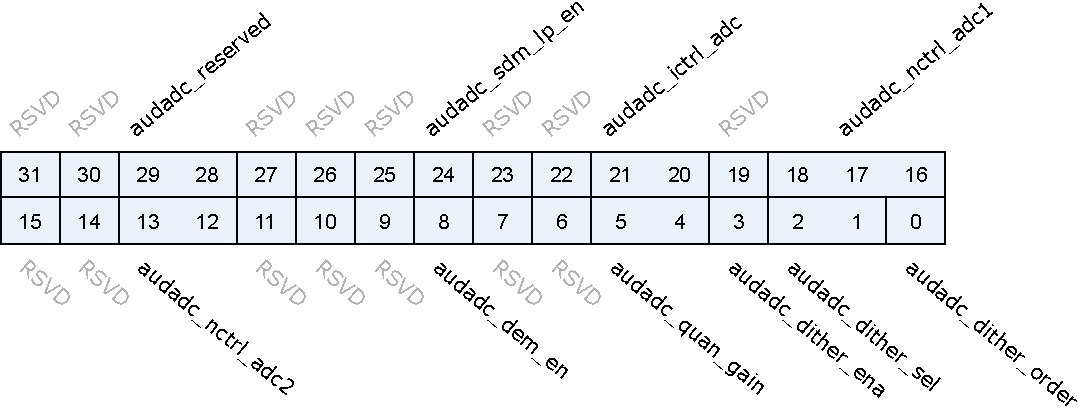
\includegraphics{ausolo_audadc_ana_cfg2.pdf}
\end{figure}

\regdes{31:30&RSVD& & & \\\hline
29:28&audadc\_reserved&r/w&2'h0&AUDADC reserved register\\\hline
27:25&RSVD& & & \\\hline
24&audadc\_sdm\_lp\_en&r/w&1'h0&SDM lowpower funciton \par 0 = disable    \par 1 = enable, 0.6 of disable
\\\hline
23:22&RSVD& & & \\\hline
21:20&audadc\_ictrl\_adc&r/w&2'h1&SDM bias current control \par 00 = 4uA          01 = 5uA \par 10 = 6uA          11 = 7uA
\\\hline
19&RSVD& & & \\\hline
18:16&audadc\_nctrl\_adc1&r/w&3'h3&op number control for first integrator in SDM \par 000 = 1(12uA)          001 = 2(24uA) \par 010 = 3(36uA)          011 = 4(48uA) \par 100 = 5(60uA)          101 = 5(60uA) \par 110 = 5(60uA)          111 = 5(60uA)
\\\hline
15:14&RSVD& & & \\\hline
13:12&audadc\_nctrl\_adc2&r/w&2'h1&op number control for second integrator in SDM \par 00 = 1(12uA)          01 = 2(24uA) \par 10 = 3(36uA)          11 = 3(36uA)
\\\hline
11:9&RSVD& & & \\\hline
8&audadc\_dem\_en&r/w&1'h1&dem function control \par 0 = disable        1 = enable
\\\hline
7:6&RSVD& & & \\\hline
5:4&audadc\_quan\_gain&r/w&2'h1&quantizer gain control for SDM \par 00 = Vref/14          01 = Vref/12 \par 10 = Vref/10          11 = Vref/8
\\\hline
3&audadc\_dither\_ena&r/w&1'h1&dither control \par 0 = disable        1 = enable
\\\hline
2:1&audadc\_dither\_sel&r/w&2'h2&dither level control for SDM \par 00 = 0                      01 = LSB*1/15 \par 10 =  LSB*2/15      11 =  LSB*3/15
\\\hline
0&audadc\_dither\_order&r/w&1'h0&dither order control for SDM \par 0 = 0 order        1 = 1 order
\\\hline

}
\subsection{audadc\_cmd}
\label{ausolo-audadc-cmd}
Address:0x2000ac68
 \begin{figure}[H]
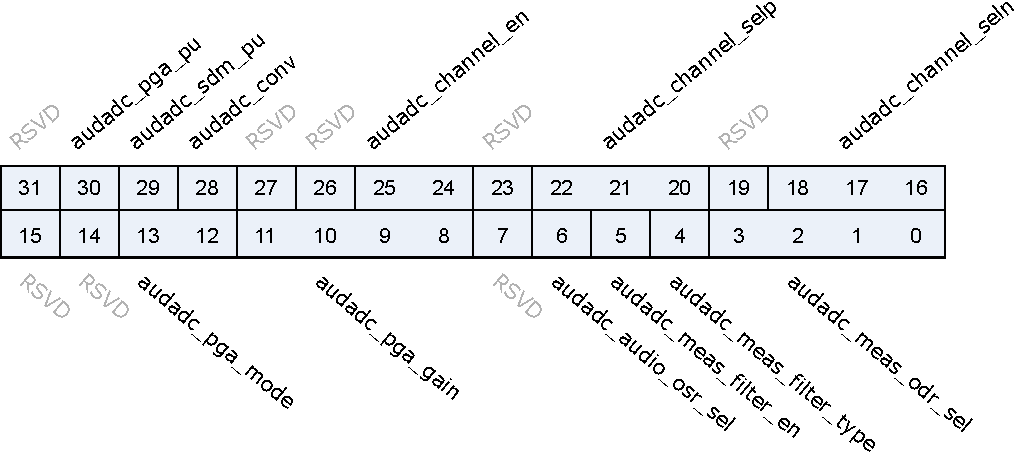
\includegraphics{ausolo_audadc_cmd.pdf}
\end{figure}

\regdes{31&RSVD& & & \\\hline
30&audadc\_pga\_pu&r/w&1'h0&PGA related circuit enable \par 0 = disable        1 = enable
\\\hline
29&audadc\_sdm\_pu&r/w&1'h0&SDM related circuit enable \par 0 = disable        1 = enable
\\\hline
28&audadc\_conv&r/w&1'h0&SDM conversion start singal \par 0 = remain resetting status        1 = start conversion \par both analog intetrator and measuring digitial decimation filter will be reset when \par audadc\_conv configured to low. Measuring digital decimation filter need to reset \par to same initial condition because it's feedback configuration for FIR. Audio filter \par dont need this resetting.
\\\hline
27:26&RSVD& & & \\\hline
25:24&audadc\_channel\_en&r/w&2'h0&channel mux switch enable or disable \par MSB controls Positive channel, LSB controls Negative channel \par 0 = disable, look into each channel will see high impedance \par 1 = enable, one of eight channel will be choose
\\\hline
23&RSVD& & & \\\hline
22:20&audadc\_channel\_selp&r/w&3'h0&Positive channel selection, connected to PGA positive terminal \par 000 = AIN0          001 = AIN1 \par 010 = AIN2          011 = AIN3 \par 100 = AIN4          101 = AIN5 \par 110 = AIN6          111 = AIN7
\\\hline
19&RSVD& & & \\\hline
18:16&audadc\_channel\_seln&r/w&3'h0&Negative channel selection, connected to PGA negative terminal \par 000 = AIN0          001 = AIN1 \par 010 = AIN2          011 = AIN3 \par 100 = AIN4          101 = AIN5 \par 110 = AIN6          111 = AIN7
\\\hline
15:14&RSVD& & & \\\hline
13:12&audadc\_pga\_mode&r/w&2'h0&PGA mode configuration \par 00: AC-Coupled \& differential-ended, Audio application \par 01: AC-Coupled \& single-ended, Audio application \par 10: DC-Coupled \& differential-ended, Measuring application \par 11: DC-Coupled \& single-ended, Measuring application(may not used)
\\\hline
11:8&audadc\_pga\_gain&r/w&4'h0&PGA Gain control \par 0000 = 6dB         0001 = 6dB \par 0010 = 6dB         0011 = 9dB \par 0100 = 12dB       0101 = 15dB \par 0110 = 18dB       0111 = 21dB \par 1000 = 24dB       1001 = 27dB \par 1010 = 30dB       1011 = 33dB \par 1100 = 36dB       1101 = 39dB \par 1110 = 42dB       1111 = 42dB
\\\hline
7&audadc\_audio\_filter\_en&r/w&1'h0&audio mode enable, audio filter is on when set to high \par 0 = disable        1 = enable
\\\hline
6&audadc\_audio\_osr\_sel&r/w&1'h0&audio osr configuration \par 0 = 128               1 = 64
\\\hline
5&audadc\_meas\_filter\_en&r/w&1'h0&measuring mode enable, measuring filter is on when set to high \par 0 = disable        1 = enable
\\\hline
4&audadc\_meas\_filter\_type&r/w&1'h0&digital dicimation filter selection when in measuring mode \par 0 = SINC3        1 = Low-Latency
\\\hline
3:0&audadc\_meas\_odr\_sel&r/w&4'h3&audadc ouput data rate selection when configured to measuring mode \par 0000 = 2.5SPS          0001 = 5SPS \par 0010 = 10SPS           0011 = 20SPS \par 0100 = 25SPS           0101 = 50SPS \par 0110 = 100SPS         0111 = 200SPS \par 1000 = 400SPS         1001 = 800SPS \par 1010 = 1000SPS       1011 = 2000SPS \par 1100 = 4000SPS       1101 = 4000SPS \par 1110 = 4000SPS       1111 = 4000SPS
\\\hline

}
\subsection{audadc\_data}
\label{ausolo-audadc-data}
Address:0x2000ac6c
 \begin{figure}[H]
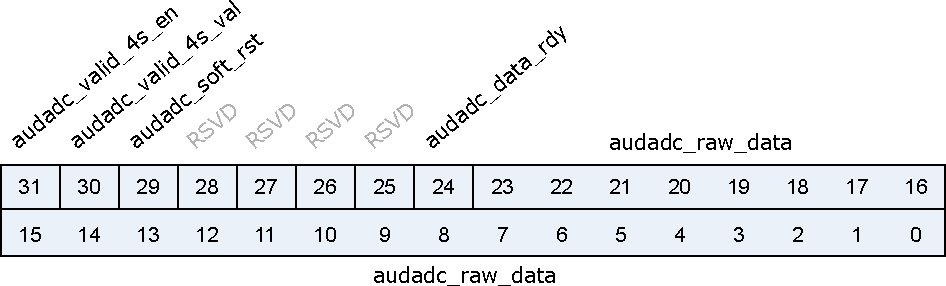
\includegraphics{ausolo_audadc_data.pdf}
\end{figure}

\regdes{31:30&RSVD& & & \\\hline
29&audadc\_soft\_rst&r/w&1'h0&don't care\\\hline
28:25&RSVD& & & \\\hline
24&audadc\_data\_rdy&r&1'h0&audadc data ready indicator when measuring mode selected, auto reset to 0 after read \par 0 = not ready       1 = ready
\\\hline
23:0&audadc\_raw\_data&r&16'h0&audadc output 16bit data, 2's\\\hline

}
\subsection{audadc\_rx\_fifo\_ctrl}
\label{ausolo-audadc-rx-fifo-ctrl}
Address:0x2000ac80
 \begin{figure}[H]
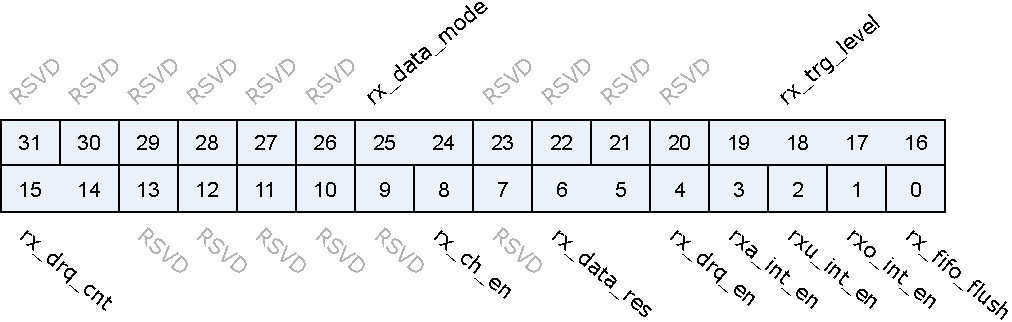
\includegraphics{ausolo_audadc_rx_fifo_ctrl.pdf}
\end{figure}

\regdes{31:26&RSVD& & & \\\hline
25:24&rx\_data\_mode&r/w&2'b0&RX\_FIFO\_DATOUT\_MODE. \par RX FIFO DATA Output Mode (Mode 0, 1, 2, 3) \par Mode 0: Valid data's MSB is at [31] of RX\_FIFO register \par Mode 1: Valid data's MSB is at [23] of RX\_FIFO register \par Mode 2: Valid data's MSB is at [19] of RX\_FIFO register \par Mode 3: Valid data's MSB is at [15] of RX\_FIFO register \par Note: Expanding ‘0’ at LSB of RX FIFO register (data invalid region) \par            Expanding sign bit at MSB of RX FIFO register (data invalid region) \par For 24-bit received audio sample resolution: \par Mode 0: RXDATA[31:0] = {FIFO\_O[23:0], 8’h0} \par Mode 1: RXDATA[31:0] = {8{FIFO\_O[23]}, FIFO\_O[23:0]} \par Mode 2: RXDATA[31:0] = {12{FIFO\_O[23]}, FIFO\_O[23:4]} \par Mode 3: RXDATA[31:0] = {16{FIFO\_O[23]}, FIFO\_O[23:8]} \par For 20-bit received audio sample resolution: \par Mode 0: RXDATA[31:0] = {FIFO\_O[23:4], 12’h0} \par Mode 1: RXDATA[31:0] = {8{FIFO\_O[23]}, FIFO\_O[23:4], 4’h0} \par Mode 2: RXDATA[31:0] = {12{FIFO\_O[23]}, FIFO\_O[23:4]} \par Mode 3: RXDATA[31:0] = {16{FIFO\_O[23]}, FIFO\_O[23:8]} \par For 16-bit received audio sample resolution: \par Mode 0: RXDATA[31:0] = {FIFO\_O[23:8], 16’h0} \par Mode 1: RXDATA[31:0] = {8{FIFO\_O[23]}, FIFO\_O[23:8], 8’h0} \par Mode 2: RXDATA[31:0] = {12{FIFO\_O[23]}, FIFO\_O[23:8], 4'h0} \par Mode 3: RXDATA[31:0] = {16{FIFO\_O[23]}, FIFO\_O[23:8]}
\\\hline
23:20&RSVD& & & \\\hline
19:16&rx\_trg\_level&r/w&4'd3&RX\_FIFO\_TRG\_LEVEL. \par RX FIFO Trigger Level (RXTL[3:0]) \par Interrupt and DMA request trigger level for RX FIFO Data Available condition \par IRQ/DRQ Generated when WLEVEL > RXTL[3:0] \par Notes: \par WLEVEL represents the number of valid samples in the RX FIFO
\\\hline
15:14&rx\_drq\_cnt&r/w&2'b0&RX\_DRQ\_CLR\_CNT. \par When RX FIFO available data less than or equal N, DRQ Request will be de-asserted. N is defined here: \par 00: IRQ/DRQ de-asserted when WLEVEL <= RXTL[3:0] \par 01: IRQ/DRQ de-asserted when WLEVEL < 1 \par 10: IRQ/DRQ de-asserted when WLEVEL < 2 \par 11: IRQ/DRQ de-asserted when WLEVEL < 4 \par WLEVEL represents the number of valid samples in the RX FIFO
\\\hline
13:9&RSVD& & & \\\hline
8&rx\_ch\_en&r/w&1'b0&RX\_FIFO\_DATIN\_SRC. \par RX FIFO Data Input Source Select. \par 0: Disable 1: Enable \par Bit8: ADC1 data
\\\hline
7&RSVD& & & \\\hline
6:5&rx\_data\_res&r/w&2'd0&RX\_SAMPLE\_BITS. \par Receiving Audio Sample Resolution \par 0: 16 bits \par 1: 20 bits \par 2: 24 bits \par 3: Reserved
\\\hline
4&rx\_drq\_en&r/w&1'b0&ADC\_DRQ\_EN. \par ADC FIFO Data Available DRQ Enable. \par 0: Disable \par 1: Enable
\\\hline
3&rxa\_int\_en&r/w&1'b0&ADC\_IRQ\_EN. \par ADC FIFO Data Available IRQ Enable. \par 0: Disable \par 1: Enable
\\\hline
2&rxu\_int\_en&r/w&1'b0&ADC\_UNDERRUN\_IRQ\_EN. \par ADC FIFO Under Run IRQ Enable \par 0: Disable \par 1: Enable
\\\hline
1&rxo\_int\_en&r/w&1'b0&ADC\_OVERRUN\_IRQ\_EN. \par ADC FIFO Over Run IRQ Enable \par 0: Disable \par 1: Enable
\\\hline
0&rx\_fifo\_flush&w1c&1'b0&ADC\_FIFO\_FLUSH. \par ADC FIFO Flush. \par Write ‘1’ to flush TX FIFO, self clear to ‘0’.
\\\hline

}
\subsection{audadc\_rx\_fifo\_status}
\label{ausolo-audadc-rx-fifo-status}
Address:0x2000ac84
 \begin{figure}[H]
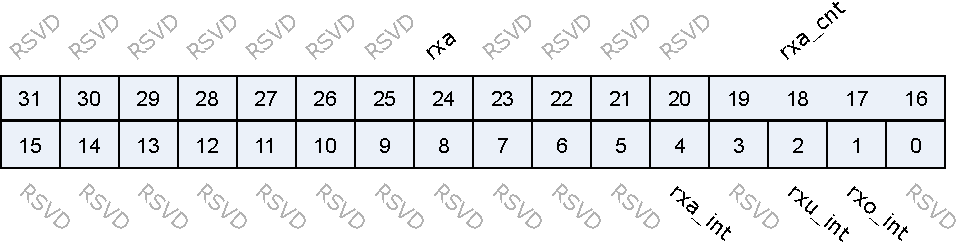
\includegraphics{ausolo_audadc_rx_fifo_status.pdf}
\end{figure}

\regdes{31:25&RSVD& & & \\\hline
24&rxa&r&1'b0&RXA. \par RX FIFO Available \par 0: No available data in RX FIFO \par 1: More than one sample in RX FIFO (>= 1 word)
\\\hline
23:20&RSVD& & & \\\hline
19:16&rxa\_cnt&r&4'h0&RXA\_CNT. \par RX FIFO Available Sample Word Counter
\\\hline
15:5&RSVD& & & \\\hline
4&rxa\_int&r&1'b0&RXA\_INT. \par RX FIFO Data Available Pending Interrupt \par 0: No Pending IRQ \par 1: Data Available Pending IRQ \par Automatic clear if interrupt condition fails.
\\\hline
3&RSVD& & & \\\hline
2&rxu\_int&r&1'b0&RXU\_INT. \par RX FIFO Underrun Pending Interrupt \par 0: No Pending IRQ \par 1: FIFO Underrun Pending IRQ \par Write ‘1’ to clear this interrupt
\\\hline
1&rxo\_int&r&1'b0&RXO\_INT. \par RX FIFO Overrun Pending Interrupt \par 0: No Pending IRQ \par 1: FIFO Overrun Pending IRQ \par Write ‘1’ to clear this interrupt
\\\hline
0&RSVD& & & \\\hline

}
\subsection{audadc\_rx\_fifo\_data}
\label{ausolo-audadc-rx-fifo-data}
Address:0x2000ac88
 \begin{figure}[H]
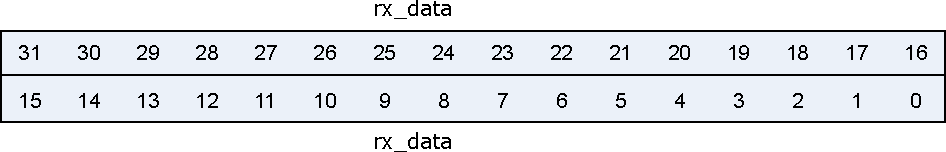
\includegraphics{ausolo_audadc_rx_fifo_data.pdf}
\end{figure}

\regdes{31:0&rx\_data&r&32'h0&RX\_DATA. \par RX Sample \par Host can get one sample by reading this register. The left channel sample data is first and then the right channel sample.
\\\hline

}
